\documentclass[12pt]{article}
\nofiles
\usepackage{graphicx}
\usepackage{umoline}
\usepackage{amssymb}
\usepackage{multido}
\usepackage{graphicx}
\usepackage{pictexwd}

\topmargin -1 in
\oddsidemargin -0.25in  % -0.25in
\evensidemargin -0.25in %-0.25in
\textheight 9.7in
\textwidth 7in

\baselineskip 20pt
\parskip 20pt
\pagestyle{myheadings}\parindent 0em

\begin{document}

\thispagestyle{empty}


\textsc{Fall 2015 General Education Assessment Problem}\\
\begin{enumerate}
\item Suppose you and your friends create a catapult and launch a coconut with it.
\begin{enumerate}
\item The height of the coconut $t$ seconds after launch is given by $f(t)=128t-16t^2$. How long will the coconut be in the air? (Here we assume it will hit the ground when the height is $0$).
\vspace{1in}
\item Viewing a graph of this function below, estimate the maximum height the coconut achieves. \vspace{.25in}\\ 
Maximum Height: \\ \vspace{.25in}
\begin{center}
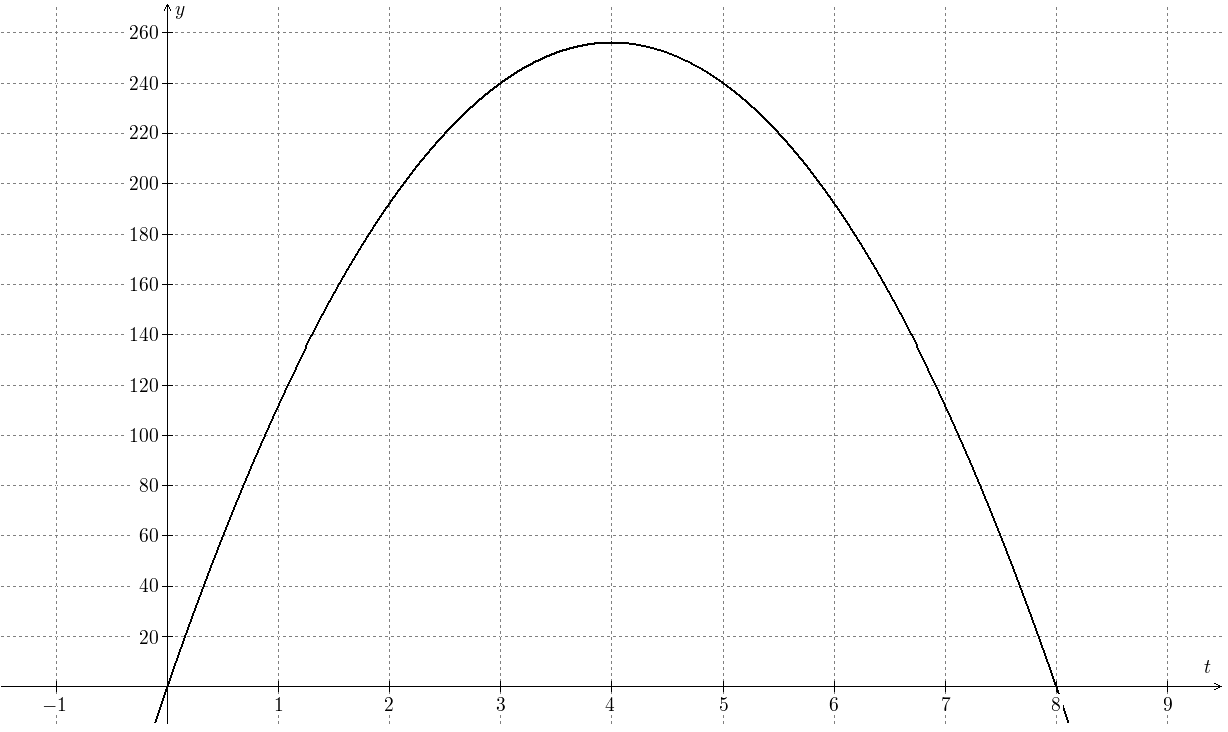
\includegraphics[scale=.5]{coconut.PNG}
\end{center}
\item Recalling that the function of the height of the coconut is $f(t)=128t-16t^2$, use your knowledge about quadratic functions to determine the actual maximum height the coconut achieves.
\end{enumerate}

\end{enumerate}

\end{document}

